\documentclass[11pt]{article}
\usepackage[margin=1in]{geometry}
\usepackage{../../styles/isaiah}
\usepackage{../../styles/components/threeBoxGrid}

\begin{document}

% Overview of Isaiah 1-12 Chiastic Structure
\isaiahChiasticOverview{5}

\newpage

% Isaiah Context Grid
\threeBoxGrid{1}{Isaiah 9:8-10:34}{
    \textbf{\large Isaiah 9:8-21}

    \textit{Anger not Turned \\Away from Israel}
}{
    \textbf{\large Isaiah 10:1-4}

    \textit{Woe to Israel \& Anger \\not Turned Away}
}{
    \textbf{\large Isaiah 10:5-34}

    \textit{Woes and Therefores \\to Assyria}
}

% Overview of Isaiah 9:8-10:27
\begin{overview}{Isaiah 9:8-9:21 — Overview}

\overviewsection[0]{%
\textbf{Verses 8-12: Nations against Israel}
}

\overviewsection[1]{%
\textbf{Verses 13-17: Israel's Leaders against Poor}
}

\overviewsection[0]{%
\textbf{Verses 18-21: Israel against Itself}
}

\end{overview}
\newpage

% Verses 8-12 - Nations against Israel
\begin{biblicaloutline}[Isaiah 9:8-12]

    \begin{versesection}{2em}
        \poetryline{\versenum{8} The Lord has sent a \sectionwordfootnote{word}{Septuigent – "plague/death"} against Jacob,}
        \poetryline{and it will fall on Israel;}
        \poetryline{\versenum{9} and all the people will know,}
        \poetryline{\highlightyellow{Ephraim} and the inhabitants of Samaria,}
        \poetryline{who say in pride and in arrogance of heart:}
        \poetryline{\versenum{10} "The bricks have fallen,}
        \poetryline{but we will build with dressed stones;}
        \poetryline{the sycamores have been cut down,}
        \poetryline{but we will put cedars in their place."}
        \poetryline{\versenum{11} But the LORD raises the adversaries of Rezin against him,}
        \poetryline{and stirs up his enemies.}
        \poetryline{\versenum{12} The Syrians on the east and the \sectionwordfootnote{Philistines on the west}{C.f. Amos 1:6 – Could be figurative or they could've been involved in capturing the fleeing Israelites during Assyrian invasion}}
        \poetryline{\highlightblue{devour} Israel with \highlightblue{open mouth}.}
        \poetryline{\highlightorange{For all this his anger has not turned away,}}
        \poetryline{\highlightorange{and his hand is stretched out still.}}
    \end{versesection}

\end{biblicaloutline}


\vspace{3em}
{\large\bfseries Bricks, Stones, Sycamores, and Cedars}
\vspace{1em}

The Bricks vs Dressed Stones and the Sycamores vs Cedars show how Israel is trying to rebuild itself after the Syro-Ephraimite War (where the Northern Kingdom fought against Judah). The bricks and sycamores are the cheap, quick, and easy way to rebuild while the dressed stones and cedars are the expensive, high quality, and long lasting way to rebuild. 

\begin{center}
\begin{minipage}[t]{0.45\textwidth}
\centering
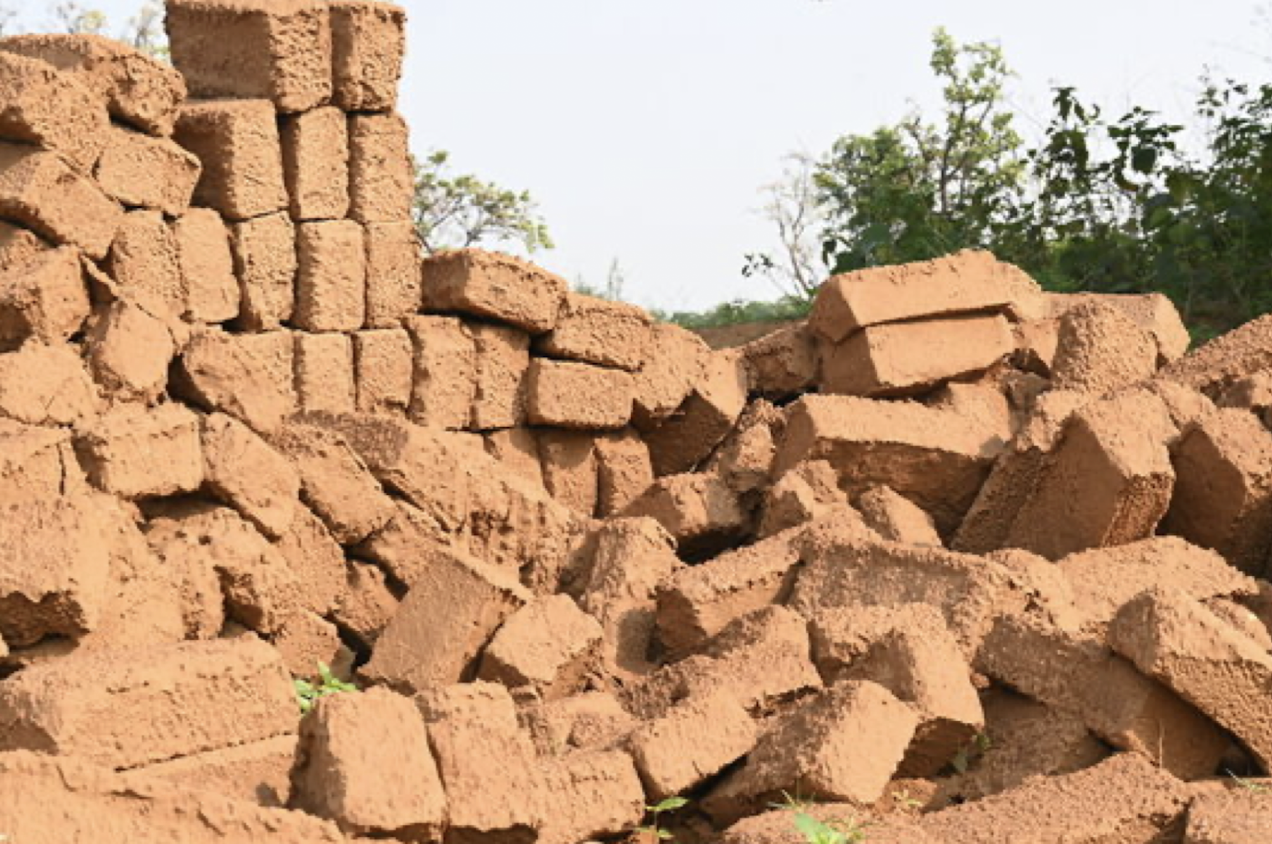
\includegraphics[width=\textwidth]{mud-bricks.png}\\
\vspace{0.5em}
Mud Bricks
\end{minipage}
\hspace{0.05\textwidth}
\begin{minipage}[t]{0.45\textwidth}
\centering
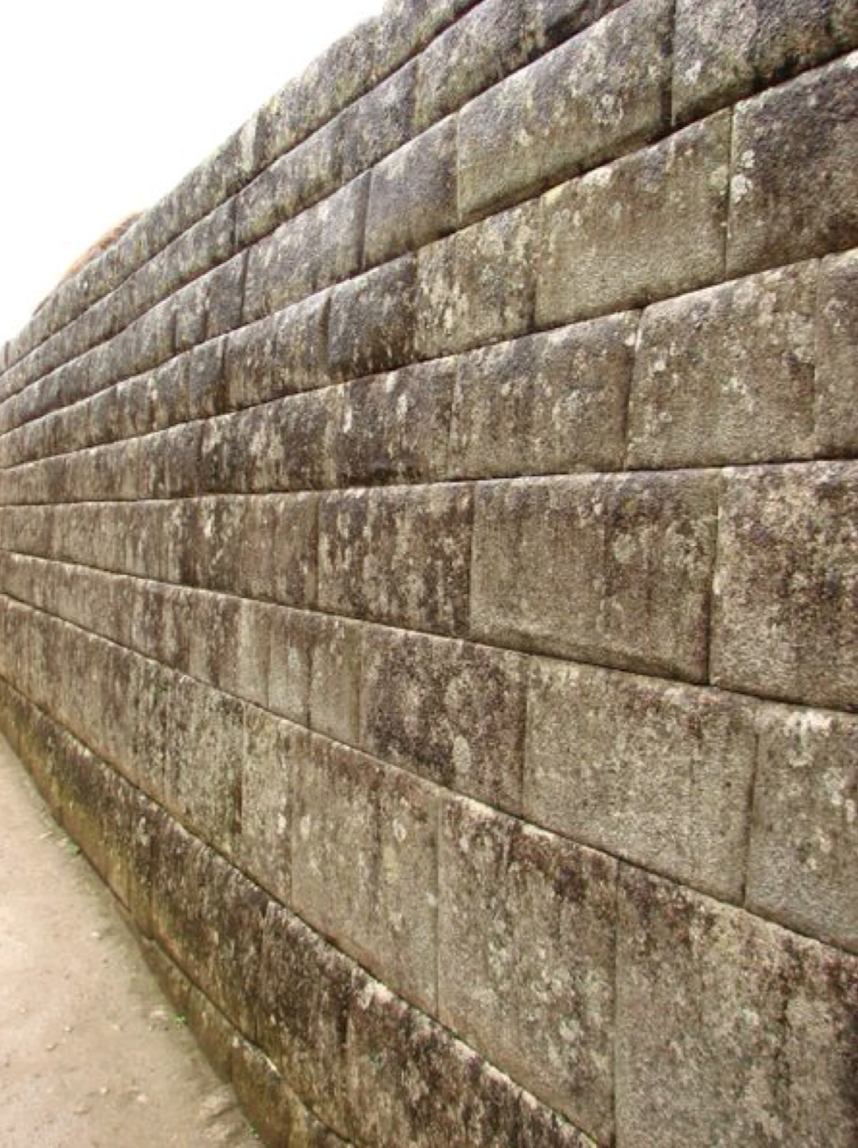
\includegraphics[width=\textwidth]{ashlar-stones.png}\\
\vspace{0.5em}
Ashlar Stones
\end{minipage}
\end{center}
\vspace{1em}

\vspace{1em}
\begin{center}
\begin{minipage}[t]{0.45\textwidth}
\centering
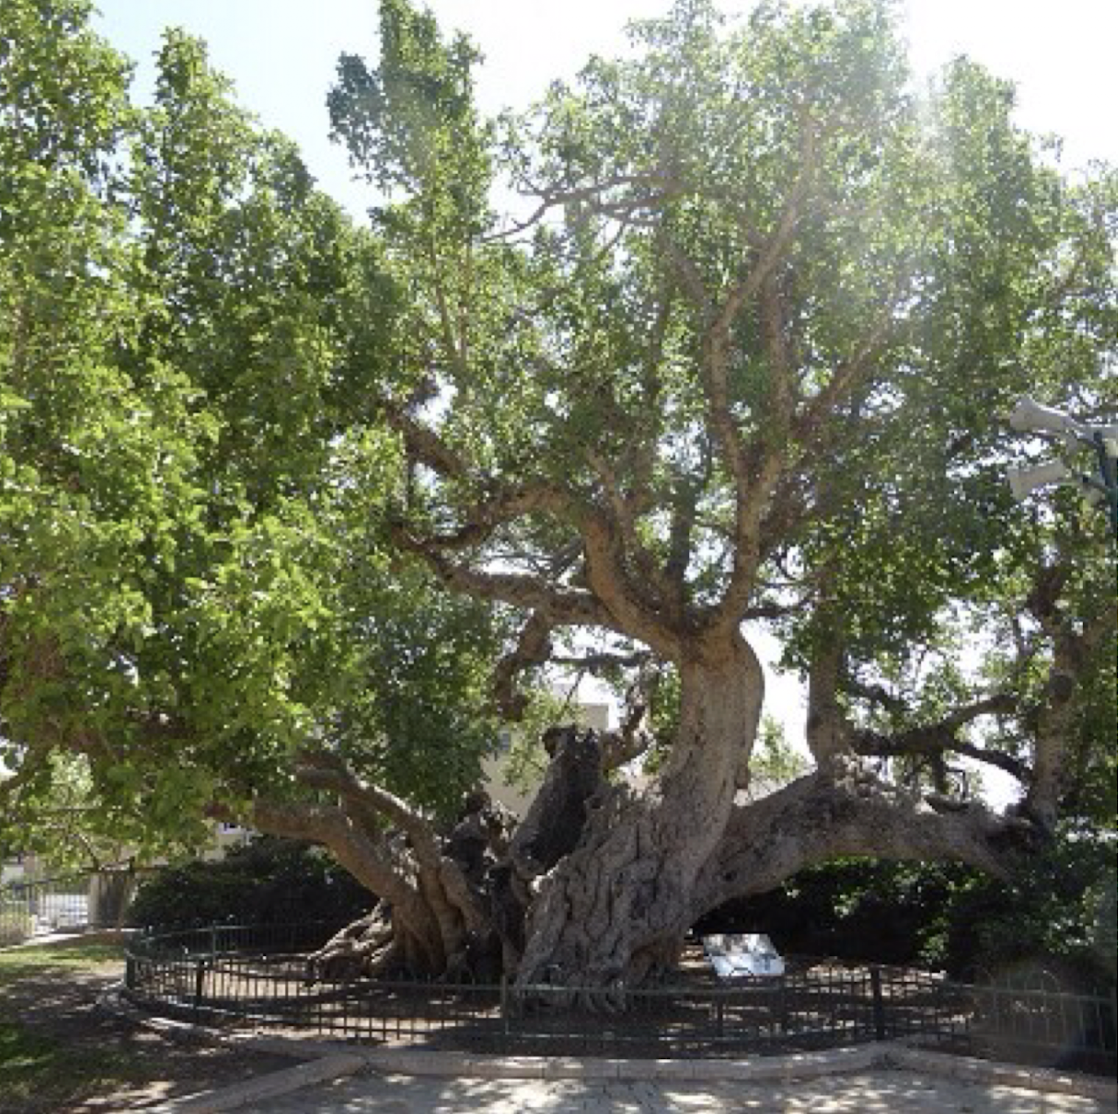
\includegraphics[width=\textwidth]{sycamore.png}\\
\vspace{0.5em}
Sycamore
\end{minipage}
\hspace{0.05\textwidth}
\begin{minipage}[t]{0.45\textwidth}
\centering
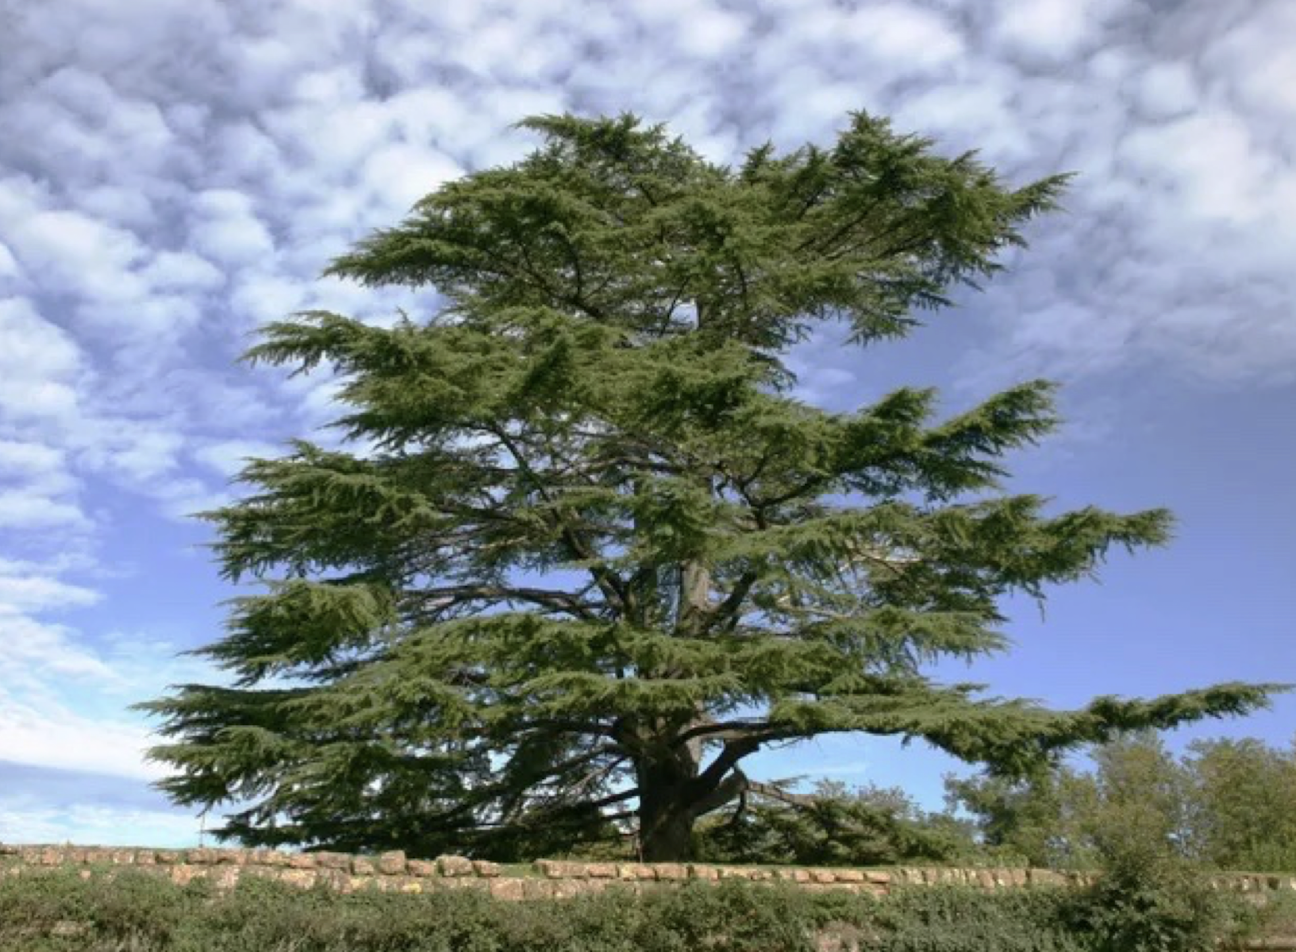
\includegraphics[width=\textwidth]{lebanon-cedar.png}\\
\vspace{0.5em}
Lebanon Cedar
\end{minipage}
\end{center}
\vspace{1em}


\newpage
{\large\bfseries "Hand Still Stretched Out"}
\vspace{1em}

The phrase "hand is stretched out still" appears throughout this passage as a refrain of divine judgment (9:12, 17, 21; 10:4). Yet elsewhere in Scripture, God's "stretched out hand" demonstrates His power to save (along with judgement on Egypt):

\begin{quote}
\textit{"Say therefore to the people of Israel, 'I am the LORD, and I will bring you out from under the burdens of the Egyptians, and I will deliver you from slavery to them, and I will redeem you with an outstretched arm and with great acts of judgment.'"}\\\\
\hfill --- Exodus 6:6
\end{quote}

\begin{quote}
\textit{"Or has any god ever attempted to go and take a nation for himself from the midst of another nation, by trials, by signs, by wonders, and by war, by a mighty hand and an outstretched arm, and by great deeds of terror, all of which the LORD your God did for you in Egypt before your eyes?"}\\\\
\hfill --- Deuteronomy 4:34
\end{quote}

The same divine hand that delivered Israel from Egypt now remains stretched out—not to judge Egypt though, but to judge Israel itself!

% Verses 13-17 - Israel's Leaders against Poor
\begin{biblicaloutline}[Isaiah 9:13-17]

    \begin{versesection}{2em}
        \poetryline{\versenum{13} The people did not turn to him who struck them,}
        \poetryline{nor inquire of the LORD of hosts.}
        \poetryline{\versenum{14} So the LORD cut off from Israel head and tail,}
        \poetryline{palm branch and reed in one day—}
        \poetryline{\versenum{15} the elder and honored man is the head,}
        \poetryline{and the prophet who teaches lies is the tail;}
        \poetryline{\versenum{16} for those who guide this people have been leading them astray,}
        \poetryline{and those who are guided by them are \highlightblue{swallowed up}.}
        \poetryline{\versenum{17} Therefore the Lord does not rejoice over their young men,}
        \poetryline{and has no compassion on their \highlightpurple{fatherless} and \highlightpurple{widows};}
        \poetryline{for everyone is godless and an evildoer,}
        \poetryline{and every \highlightblue{mouth} speaks folly.}
        \poetryline{\highlightorange{For all this his anger has not turned away,}}
        \poetryline{\highlightorange{and his hand is stretched out still.}}
    \end{versesection}

\end{biblicaloutline}

\newpage
{\large\bfseries "Devoured"}
\vspace{1em}

Seeing the repeated phrases around \highlightblue{eating}/\highlightblue{swallowing up}, we can see what Israel's leaders are doing to their vulnerable is put on analogy to what the Syrians and Philistines are doing to Israel and what they will ultimately do to each other. Thinking through how they must have viewed their enemies around them that are ravaging their homes and killing their people, the Lord turns that right around back on them! That's how they're treating the most vulnerable in their communities!


\vspace{3em}
{\large\bfseries God has no compassion on Poor?}
\vspace{1em}

The opposite of taking care of them is teaching lies and leading astray. Even those who are supposed to be cared for are led to moral corruption by the leaders. This is kind of like how the prosperity gospel of today feeds on the vulnerable and leads them away from the truth.

% Verses 18-21 - Israel against Itself
\begin{biblicaloutline}[Isaiah 9:18-21]

    \begin{versesection}{2em}
        \poetryline{\versenum{18} For wickedness burns like a \highlightred{fire};}
        \poetryline{it \highlightblue{devours} briers and thorns;}
        \poetryline{it kindles the thickets of the forest,}
        \poetryline{and they roll upward in a column of smoke.}
        \poetryline{\versenum{19} Through the wrath of the LORD of hosts}
        \poetryline{the land is scorched,}
        \poetryline{and the people are like fuel for the \highlightred{fire};}
        \poetryline{no one spares another.}
        \poetryline{\versenum{20} They slice meat on the right, but are still hungry,}
        \poetryline{and they \highlightblue{devour} on the left, but are not satisfied;}
        \poetryline{each \highlightblue{devours} the flesh of his own \sectionwordfootnote{arm}{Septuigent – "Brother"; Could also be interpreted "seed"}:}
        \poetryline{\versenum{21} Manasseh \highlightblue{devours} \highlightyellow{Ephraim}, and \highlightyellow{Ephraim} Manasseh;}
        \poetryline{and together they are against Judah.}
        \poetryline{\highlightorange{For all this his anger has not turned away,}}
        \poetryline{\highlightorange{and his hand is stretched out still.}}
    \end{versesection}

\end{biblicaloutline}

\vspace{3em}
{\large\bfseries Who's Doing This?}
\vspace{1em}

In verses 18-21 we see a pattern that started all the way back in the early chapters of Genesis: God's wrath being evidenced as handing people over to their own destructive desires. Consider the flood narrative:

\begin{quote}
\textit{"The LORD saw that the wickedness of man was great in the earth, and that every intention of the thoughts of his heart was only evil continually... Now the earth was corrupt in God's sight, and the earth was filled with violence."}\\\\
\hfill --- Genesis 6:5, 11
\end{quote}

God's judgment in Genesis wasn't arbitrary—He allowed humanity's violence to run its full course until it consumed them. Similarly, in Isaiah 9:18-21, wickedness "burns like a fire" and the people become "fuel for the fire" (v. 19). They devour one another—Manasseh against Ephraim, Ephraim against Manasseh—in an insatiable cycle of self-destruction. God's wrath is demonstrated not by direct intervention but by removing His restraining hand and allowing their wickedness to consume them from within. This is the terrifying reality of divine judgment: sometimes God simply gives people over to what they already desire, and they destroy themselves.

\end{document}
